\documentclass[tikz,border=2mm]{standalone}
\usepackage{tikz}
\usetikzlibrary{calc}

\begin{document}
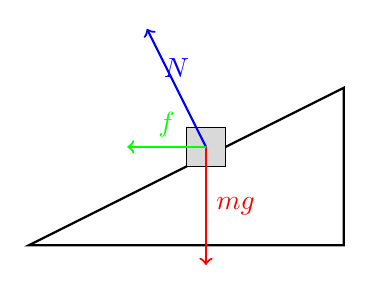
\begin{tikzpicture}

% Draw inclined plane
\draw[thick] (0,0) -- (4,2) -- (4,0) -- cycle;

% Draw block
\path[draw, fill=gray!30] (2,1) rectangle ++(0.5, 0.5);

% Draw forces
\draw[->, red, thick] (2.25, 1.25) -- ++(0, -1.5) node[midway,right] {$mg$}; % Gravity
\draw[->, blue, thick] (2.25, 1.25) -- ++(-0.75, 1.5) node[midway,above] {$N$}; % Normal force
\draw[->, green, thick] (2.25, 1.25) -- ++(-1, 0) node[midway,above] {$f$}; % Friction

\end{tikzpicture}
\end{document}